% Created 2019-07-12 ven. 17:46
% Intended LaTeX compiler: pdflatex
\documentclass[11pt]{article}
\usepackage[utf8]{inputenc}
\usepackage[T1]{fontenc}
\usepackage{graphicx}
\usepackage{grffile}
\usepackage{longtable}
\usepackage{wrapfig}
\usepackage{rotating}
\usepackage[normalem]{ulem}
\usepackage{amsmath}
\usepackage{textcomp}
\usepackage{amssymb}
\usepackage{capt-of}
\usepackage{hyperref}
\author{helenon}
\date{\today}
\title{}
\hypersetup{
 pdfauthor={helenon},
 pdftitle={},
 pdfkeywords={},
 pdfsubject={},
 pdfcreator={Emacs 25.2.2 (Org mode 9.2.3)}, 
 pdflang={English}}
\begin{document}


\section*{Experiment : evaluate grasping precision and repeatability}
\label{sec:org1f6fba8}

\begin{itemize}
\item Experiment presentation
\label{sec:org8494474}
ool
\begin{center}
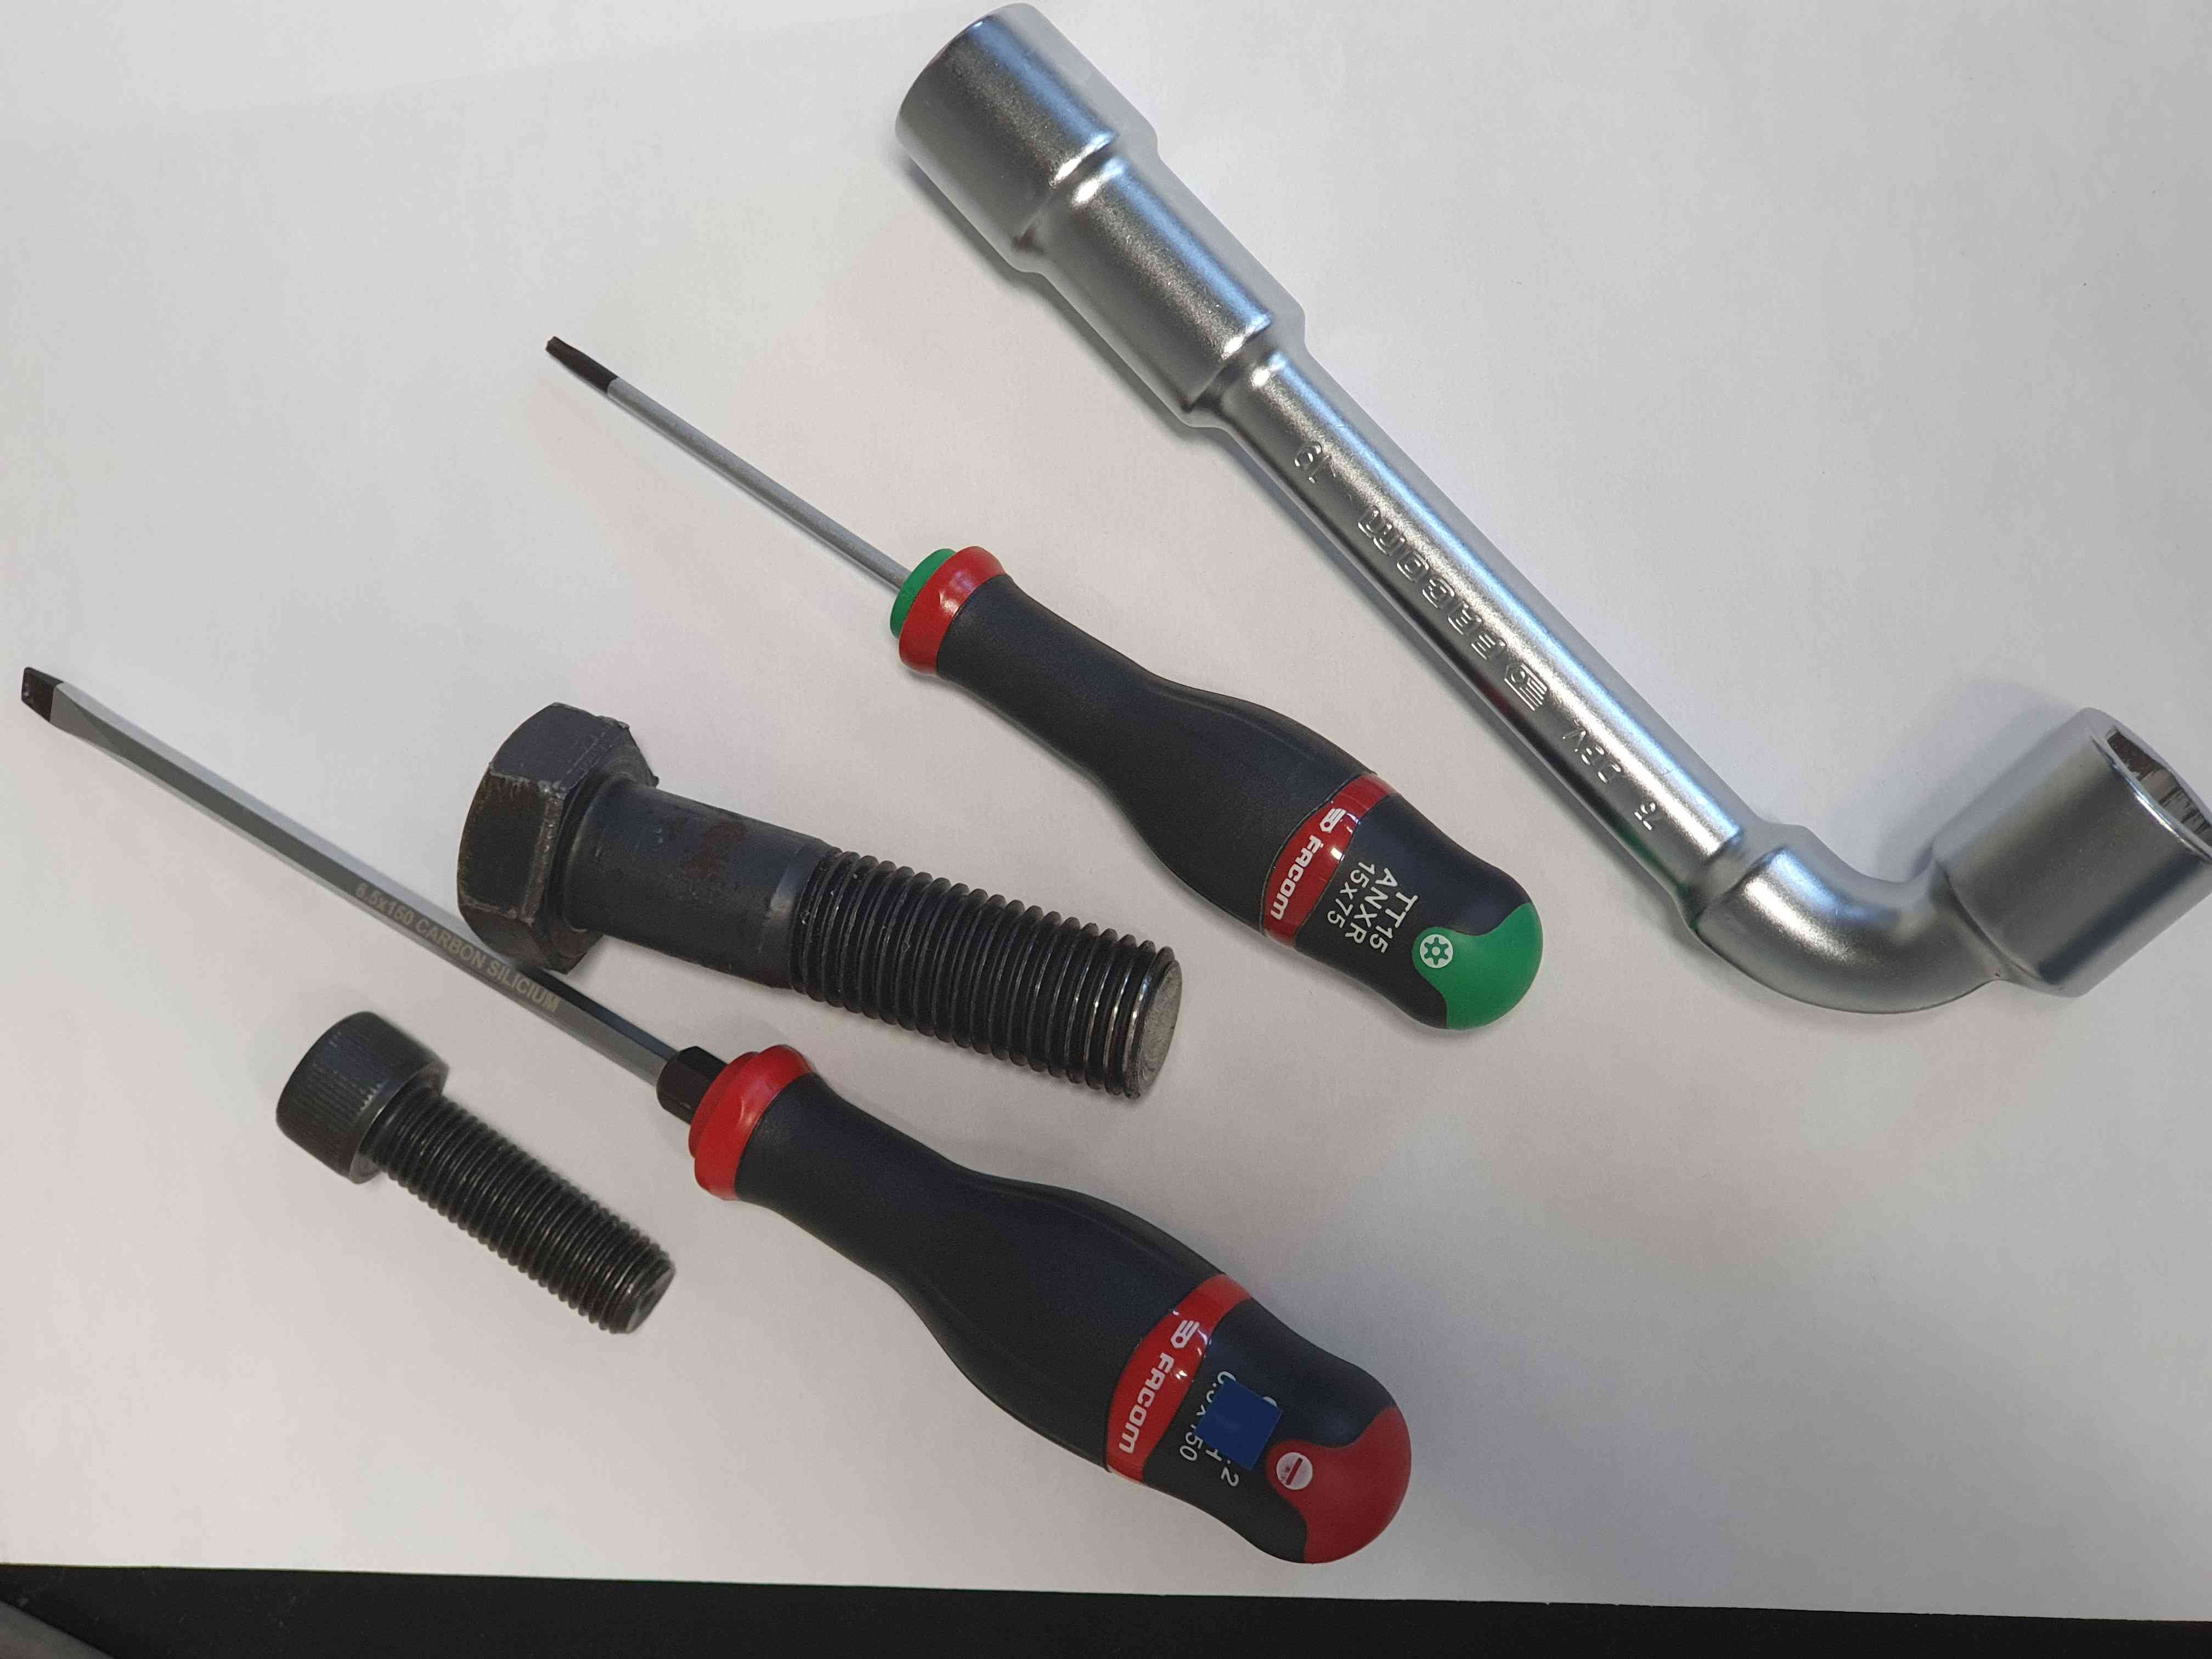
\includegraphics[width=.9\linewidth]{./jeu-outils.jpg}
\label{fig:outils}
\end{center}


\begin{figure}[htbp]
\centering
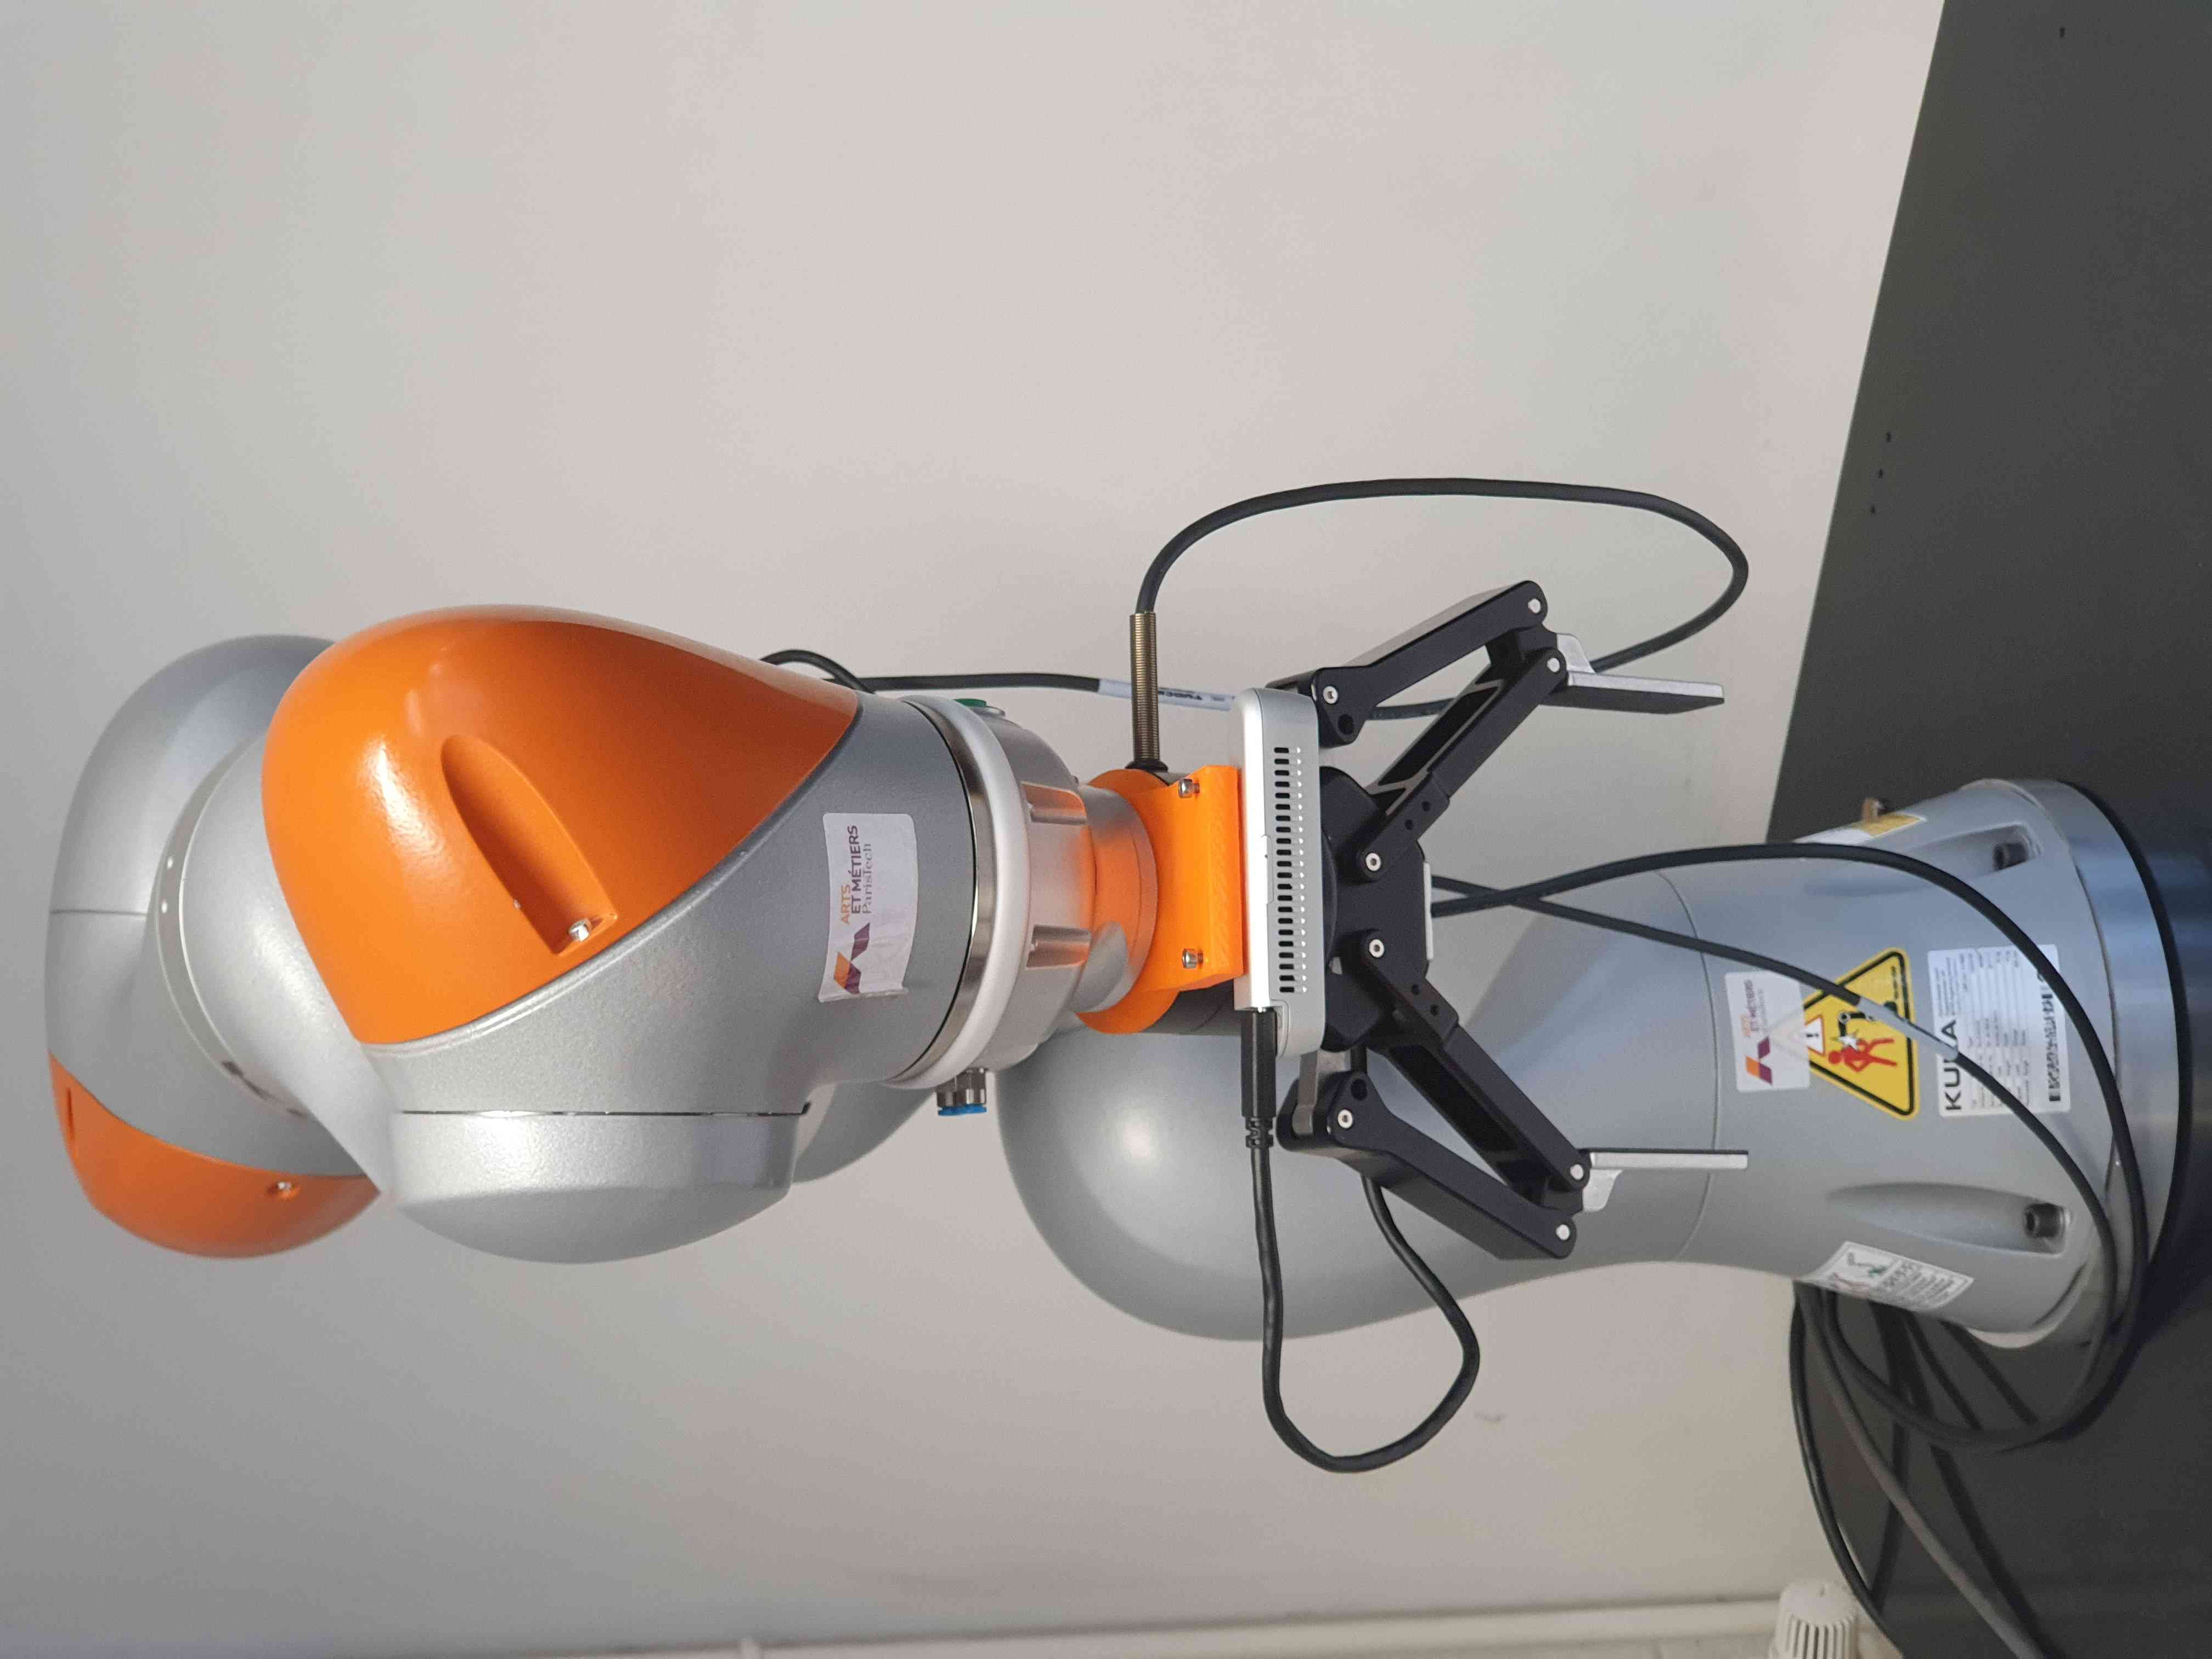
\includegraphics[width=.9\linewidth]{./iiwa_intel.jpg}
\caption{\label{fig:iiwa}
Robot configuration}
\end{figure}

\begin{figure}[htbp]
\centering
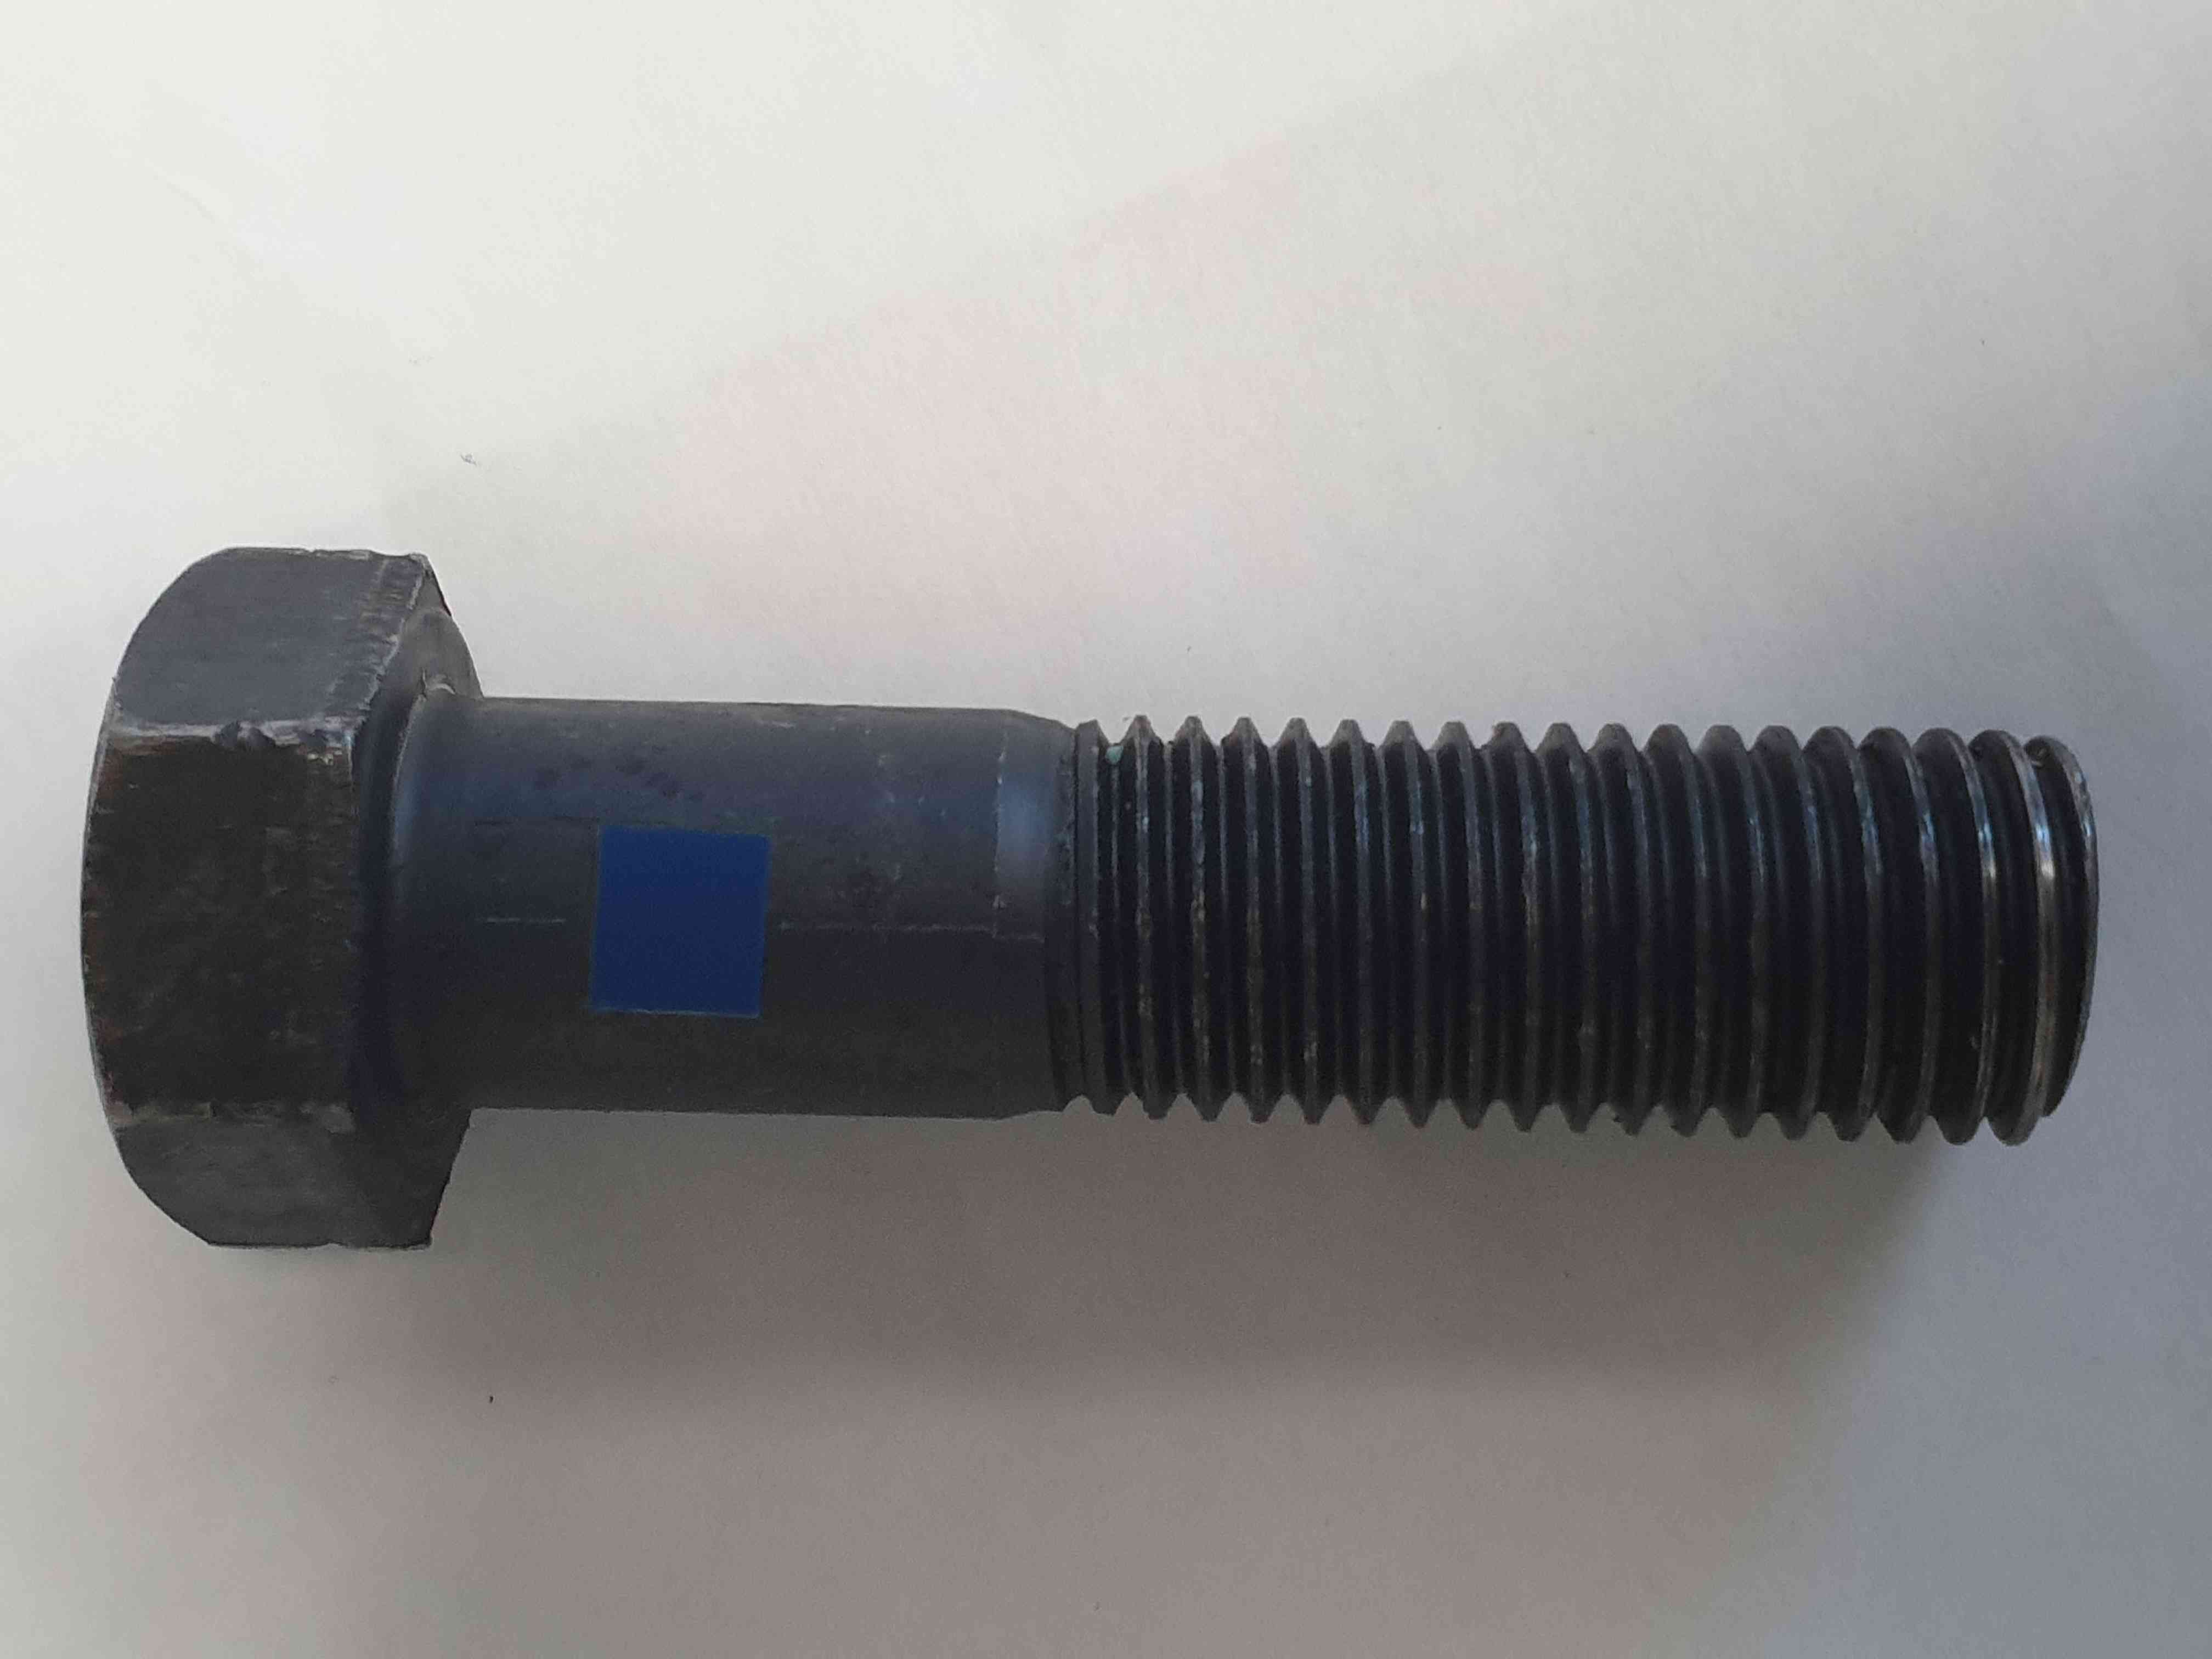
\includegraphics[width=.9\linewidth]{./vis_libellee.jpg}
\caption{\label{fig:adhesive}
In order to ease measurement colored adhesive are used as a reference point. Thus one can bypass curbersome CAD reconstruction based on the cloud point.}
\end{figure}
\end{itemize}
\end{document}